% ----------------------------------------------------------------------------
% 
% ----------------------------------------------------------------------------

\documentclass[11pt, parskip=half]{scrartcl}       % KOMA-Skript für Artikel

%% Präambel
\usepackage[english, ngerman]{babel} % deutsche typogr. Regeln + Trenntabelle
\usepackage[T1]{fontenc}             % interner TeX-Font-Codierung
\usepackage{lmodern}                 % Font Latin Modern
\usepackage[utf8]{inputenc}          % Font-Codierung der Eingabedatei
\usepackage[babel]{csquotes}         % Anführungszeichen
\usepackage{graphicx}                % Graphiken
\usepackage{booktabs}                % Tabellen schöner
\usepackage{amsmath}      % Mathematik
\usepackage{amssymb}      % Mathematische Symbole
\usepackage{float}
\usepackage[pdftex]{hyperref}
\usepackage{subcaption}
\usepackage{url}
\hypersetup{
  bookmarksopen=true,
  bookmarksopenlevel=3,
  colorlinks,
  citecolor=blue,
  linkcolor=blue
}
\usepackage{scrhack} % unterdrückt Fehlermeldung von listings

%% Nummerierungstiefen
\setcounter{tocdepth}{3}     % 3 Stufen im Inhaltsverzeichnis
\setcounter{secnumdepth}{3}  % 3 Stufen in Abschnittnummerierung

\newcommand*{\N}{\mathbb{N}}
\newcommand*{\Z}{\mathbb{Z}}
\newcommand*{\Q}{\mathbb{Q}}
\newcommand*{\R}{\mathbb{R}}

% Code packages
\usepackage{listingsutf8} % Code mit UTF-8 Support
\usepackage{color,xcolor} % Farben definierbar als HTML, RGB, ...
\usepackage{textcomp}

\definecolor{alabasterGray}{HTML}{F7F7F7}
\definecolor{alabasterBlue}{HTML}{325CC0}
\definecolor{alabasterGreen}{HTML}{448C27}
\definecolor{alabasterPink}{HTML}{7A3E9D}
\definecolor{alabasterRed}{HTML}{AA3731}

\lstset{ 
  basewidth={0.5em,0.45em},
  extendedchars=true,
  backgroundcolor=\color{alabasterGray}, % background color (color or xcolor needed)
  basicstyle=\small\ttfamily, 
  keywordstyle=\color{alabasterBlue}, 
  commentstyle=\color{alabasterRed}, 
  rulecolor=\color{black},          % frame color may change if not set (frame on comment, is comment-colored)
  stringstyle=\color{alabasterGreen}, 
  numberstyle=\tiny\color{gray},    % 
  numbers=none,                     % where to put the line-numbers (none, left, right)
  numbersep=7pt,                    % margin between numbers and code
  stepnumber=1,                     % every n-th row will be numbered
  captionpos=b,                     % sets the caption-position to bottom
  frame=single,	                    % adds a frame around the code 
  keepspaces=true,                  % keeps spaces in text
  showtabs=false,                   % show tabs as special char
  showspaces=false,                 % show spaces as special char
  showstringspaces=false,           % show spaces in strings only as special char
  tabsize=2,	                    % tabsize is 2 spaces
  breakatwhitespace=false,          % sets if automatic breaks should only happen at whitespace
  breaklines=true,                  % sets automatic line breaking
}
\lstset{
  literate={ö}{{\"o}}1
           {ä}{{\"a}}1
           {ü}{{\"u}}1
           % https://tex.stackexchange.com/questions/17739/listings-package-how-to-highlight-math-operators
           {true}{{{\color{alabasterPink}true}}}4
           {false}{{{\color{alabasterPink}false}}}5
           {TRUE}{{{\color{alabasterPink}TRUE}}}4
           {FALSE}{{{\color{alabasterPink}FALSE}}}5
           {True}{{{\color{alabasterPink}True}}}4
           {False}{{{\color{alabasterPink}False}}}5
}

\begin{document}

\titlehead{
\includegraphics[width=\textwidth]{src/Logo_THM_CG_FB06.png}}

%% Titelseite
\subject{Manusskript}
\title{Rechenzeitvergleich verschiedener Ausführungsmodelle}
\subtitle{Kurs \enquote{Wissenschaftliches Arbeiten in der Informatik}}
\author{Niklas Deworetzki}
\date{13. Mai 2019}
\maketitle

\vspace*{1.5cm}
\section*{\centerline{Zusammenfassung}}

Diese Arbeit befasst sich mit den Unterschieden in der Rechenzeit herkömmlicher Ausführungsmodelle.
Dabei werden die Programmiersprachen Haskell, Java und Python verwendet, die stellvertretend für die drei verschiedenen Ausführungsmodelle ``kompilierter Maschinencode'', ``spezifischer Zwischencode für eine virtuelle Maschine'' und ``interpretierter Quellcode'' stehen.
Der Fokus liegt dabei auf der Rechenzeit, die für das Ausführen der Berechnungen oder eines ganzen Programms benötigt wird.
Vor- und Nachteile der jeweiligen Sprachen und benötigten Sprachtransformationen werden nur für die Interpretation der Messwerte herangezogen.
Ergebnis dieser Arbeit ist, dass kein Ausführungsmodell generell als überlegen bezeichnet werden kann und je nach Anspruch der Berechnungen die Vor- und Nachteile eines Ausführungsmodells abegwägt werden müssen.                                                             

\newpage

\tableofcontents
\newpage

\section{Einleitung}

Bei der Implementierung eines Algorithmus ist es häufig wichtig, dass dieser möglichst wenig Rechenzeit benötigt, damit dieser auch für große Eingabewerte in annehmbarer Zeit ein Ergebnis liefert.
Oft werden daher als Ausführungsmodell kompilierte Maschineninstruktionen gewählt, in der Hoffnung eine geringere Rechenzeit zu erhalten.
Dabei geht jedoch häufig der Zugriff auf Features der höheren Abstraktionsebenen verloren, die bei interpretiertem Quellcode oder der Ausführung von Zwischencode auf einer virtuellen Maschine verfügbar sind.
Der Frage, ob sich dieser Kompromiss lohnt, wird in dieser Arbeit anhand konkreter Rechenzeiten diskutiert.

Dabei werden zunächst die allgemeinen Vor- und Nachteile der verschiedenen Ausführungsmodelle angeführt und versucht ein gemeinsamer Nenner zu finden, der als Grundlage für den Vergleich der Modelle dienen soll.
Als Vertreter der Ausführungsmodelle werden Haskell, Java und Python gewählt.
Quellcode in Haskell wird zu nativen Maschineninstruktionen kompiliert, während Quellcode in Java zu einem speziellen Zwischencode kompiliert wird, der für die ``Java Virtual Machine'' optimiert ist.
Python kann Quellcode mit Hilfe eines Interpreters in unveränderter Form ausführen.
Als Grundlage für einen Vergleich bietet sich die Berechnung der Fibonacci-Zahlen an.
Die benötigte Rechenzeit zum bestimmen der Fibonacci-Zahlen wird in dieser Arbeit auf zwei Arten bestimmt.
Es wird nicht nur die bloße Rechenzeit der Funktionen gemessen, sondern auch die Zeit, die für das Starten, Laden und Einrichten der Laufzeitumgebung benötigt wird, da diese Faktoren zusätzlich einen Einfluss auf die Laufzeit einer Berechnung hat.


\section{Moderne Ausführungsmodelle}

Im Folgenden werden verschiedene Ausführungsmodelle diskutiert.
Ein Ausführungsmodell beschreibt, wie ein Programm aus einer Quellsprache transformiert werden muss, um es in eine ausführbare Form zu bringen und wie der Prozess des Ausführens abläuft.\cite{execution_systems}
Einzelheiten des Transformierens sowie des Ausführens können sich dabei zwischen den konkreten Quellsprachen stark unterscheiden, wodurch nur eine allgemeine Diskussion möglich ist.

\subsection{Ausführbarer Maschinencode}

Das erste hier diskutierte Ausführungsmodell ist Maschinencode, welcher in direkt ausführbaren Dateien gespeichert wird.
Programmiersprachen wie C, C++ oder auch Haskell werden normalerweise zu ausführbaren Dateien kompiliert, die das ursprüngliche Programm in Form von plattformabhängigen Instruktionen enthält.
Diese Instruktionen können direkt in den Hauptspeicher geladen und dort vom entsprechenden Prozessor ausgeführt werden.

Dieses Modell ermöglicht ein sehr effizientes Ausführen, da nach dem Laden der Instruktionen in den Hauptspeicher direkt mit der Ausführung eines Programms begonnen werden kann, ohne auf abhängige Prozesse oder Umgebungen warten zu müssen.
Zudem können plattformabhängige Ressourcen effizient genutzt werden, da der Maschinencode speziell auf diese zugeschnitten wird, wodurch kompilierte Programme normalerweise sehr schnell sind und wenig Arbeitsspeicher benötigen.
Durch das Kompilieren wird Code der Quellsprache mehreren Analyseschritten\cite{advanced_compiler_design} unterzogen, die Optimierungen ermöglichen, was sowohl Geschwindigkeit als auch Ressourcenverbrauch zusätzlich verbessern kann.
Durch diese Analyseschritte ist es auch möglich, Programmierfehler vorab zu erkennen.

Als Nachteil bei diesem Modell muss jedoch der verhältnismäßig hohe Aufwand bei der Erzeugung des Maschinencodes beachtet werden.
Ein Compiler muss für jede Maschinenarchitektur angepasst werden, um die gegebenen Ressourcen und maschinenspezifischen Prozessoranweisungen auch nutzen zu können.
Ein anderer Nachteil wird bei der Softwareentwicklung deutlich.
Änderungen führen immer einen neuen Kompiliervorgang mit sich, wodurch die Entwicklung verlangsamt wird.
Zudem ist es schwerer, Fehler während der Laufzeit ausfindig zu machen, da nur Maschinencode vorliegt, der keine der ursprünglichen Bezeichner enthält und dessen Struktur sehr unterschiedlich zum Quellcode sein kann.
Durch den geringen Abstraktionsgrad des Maschinencodes muss häufig auf höhere Sprachfeatures verzichtet werden.\cite{quora_pros_and_cons_compiled_languages}
Beispielsweise wird die Introspektion ohne eine Laufzeitumgebung nur dadurch möglich, dass zu allen Instanzen bereits zur Kompilierzeit Typinformationen abgelegt werden.\cite{reflexive_programmiersprachen}
In C++ können für diesen Zweck Präprozessoranweisungen verwendet werden, mit deren Hilfe der Programmierer im Quellcode die benötigten Zusatzinformationen über Typen und Namen der Instanzvariablen selbst in entsprechende Strukturen eintragen kann.

\subsection{Interpretierter Quellcode}

Ein weiteres Ausführungsmodell ist das interpretierte Ausführen von Quellcode durch einen Interpreter.
Beispiele für interpretierte Programmiersprachen sind Python, JavaScript und einige Lisp-Dialekte.
Bei interpretierten Sprachen wird der Quellcode direkt geladen und von einem Interpreter ausgeführt, der einzelne Anweisungen und Ausdrücke erkennt und mit den dazugehörigen Aktionen verbindet.

Ein interpretiertes Ausführen von Quellcode hat den Vorteil, dass Sprache und Laufzeitumgebung unabhängig von der zugrundeliegenden Maschine sind.
Zudem kann der Interpreter anfallende Verwaltungsaufgaben wie Speicherverwaltung automatisch übernehmen.
Auch die Introspektion wird deutlich vereinfacht, da alle Informationen über Struktur des Programms direkt zur Laufzeit vom Interpreter erfasst und verwaltet werden können.
Python bietet beispielsweise eine Anweisung \texttt{type} an, die zu jeder Laufzeitinstanz den zugrundeliegenden Typen bestimmen kann.
Diese Zusatzinformationen zur Laufzeit sowie das Vorliegen des Quellcodes zu jeder ausgeführten Aktion erleichtert das Nachvollziehen des Programmflusses nicht nur bei der Fehlersuche enorm.
Da zudem der Schritt des Kompilierens wegfällt, wird die Softwareentwicklung deutlich beschleunigt und vereinfacht.

Die Nachteile dieses Modells gehen jedoch direkt aus den vorhin genannten Vorteilen hervor.
Mit dem fehlenden Kompiliervorgang fällt die komplette Codeanalyse weg, die mit dem Kompilieren einhergeht.
Dadurch fallen Programmierfehler wie fehlerhafte Aufrufe oder Bezeichner erst zur Laufzeit auf, wodurch interpretierte Programme fehleranfälliger werden können.
Zudem fehlen auch die Optimierungsschritte, die sonst beim Kompilieren angewandt werden, wodurch es zu Einbußen bei der Rechenzeit kommen kann.
Diese können zwar durch Just-in-time-Kompilierung teilweise zur Laufzeit nachgeholt werden, jedoch benötigt der Kompiliervorgang zur Laufzeit sowie der Interpreter selbst einige Ressourcen, sodass interpretierte Sprachen oft langsamer sind und mehr Arbeitsspeicher benötigen.\cite{stackoverflow_pros_and_cons_interpreted_languages}

\subsection{Virtuelle Maschinen und spezialisierter Zwischencode}

Das letzte Ausführungsmodell ist die Ausführung von Zwischencode durch eine virtuelle Maschinen.
Dieses Modell wird von Programmiersprachen wie Java, C\# oder Erlang verwendet.

In diesem Modell wird ein Programm aus einer Quellsprache nicht in eine maschinennahe Zielsprache kompiliert, sondern in einen spezialisierten Zwischencode, welcher von einer virtuellen Maschine ausgeführt wird und häufig Bytecode genannt wird.
Dies soll die Vorteile aus beiden vorher genannten Modellen verbinden.

Durch den vorangehenden Kompiliervorgang besteht die Möglichkeit zur Analyse des Quellcodes, wodurch Fehler vorzeitig erkannt und Optimierungen angewandt werden können.
Der erzeugte Bytecode ist auf die virtuelle Maschine zugeschnitten und ermöglicht eine schnelle Umsetzung in die entsprechenden Anweisungen.
Zusätzlich besteht die Möglichkeit zur Just-in-time-Kompilierung des Bytecodes, wobei der Zwischencode in maschinenspezifische Instruktionen übersetzt wird, wodurch die Rechenzeiten zusätzlich verringert werden.
Durch die virtuelle Maschine ist dabei eine Laufzeitumgebung gegeben, die ähnlich wie beim interpretierten Code die Speicherverwaltung übernehmen kann und zudem Informationen zu Laufzeitkonstrukten und Instanzen verwaltet, wodurch Introspektion ermöglicht wird.

Als Nachteil ist der Overhead zu sehen, der durch die komplexe virtuelle Maschine erzeugt wird.
Um die Laufzeitumgebung der virtuellen Maschine bereitzustellen, muss Arbeitsspeicher und Rechenleistung zusätzlich zum eigentlichen Programm verwendet werden.
Zudem muss die komplette virtuelle Maschine zu Programmstart initialisiert werden, was besonders bei kleineren Programmen einen Großteil der benötigten Rechenzeit ausmacht.


\section{Auswahl der Programmiersprachen}

Um einen Vergleich zwischen den vorher genannten Ausführungsmodellen möglich zu machen, müssen nun Programmiersprachen zu jedem Modell gewählt werden, die mit vergleichbaren Konstrukten umgehen können und ähnliche Unterstützung für Sprachfeatures bieten.
Zusätzlich zu Ausführungsmodellen gibt es verschiedene Paradigmen, die unterschiedliche Arten der Problemlösung mit sich führen.
Eine prozedurale Sprache wird Sprachkonstrukte für Schleifen bieten, um Datenstrukturen zu verarbeiten, während eine funktionale Sprache für solche Aufgaben Pattern-Matching und Rekursion bieten wird.
Auch die Auswahl an verschiedenen Datentypen muss berücksichtigt werden.
In den meisten Programmiersprachen gibt es für ganzzahlige Datentypen verschiedenen Größen.
Unterschiedliche Größen und Darstellungen im Hauptspeicher führen zu unterschiedlichem Rechenaufwand beim Auswerten von Rechenoperationen mit diesen Zahlen, was einen Vergleich erschwert.
Bei Gleitkommazahlen tritt eine ähnliche Problematik auf.\cite{arxiv_comparative_study_of_languages}

All diese Punkte müssen berücksichtigt werden bei der folgenden Auswahl an Programmiersprachen.

\subsection{Haskell}

Haskell ist eine rein funktionale Sprache\cite{haskell_language}, welche in mehreren Schritten zu nativem Maschinencode kompiliert wird.\cite{haskell_code_generation}
Während des Kompilierens wird Haskells starkes Typsystem für die Analyse verwendet.

Haskells Syntax ist darauf ausgerichtet, mathematische Ausdrücke und Funktionen im Quellcode darzustellen.
Dieser mathematische Schwerpunkt der Programmiersprache wird durch einen ganzzahligen Datentypen unterstützt, dessen Größe von der Architektur der Maschine abhängt, auf der das Programm ausgeführt wird.
In dieser Arbeit wird eine 64-Bit Architektur verwendet, wodurch die Größe des Zahlentyps auch 64-Bit beträgt.
Kommazahlen werden standardmäßig auch als 64-Bit Gleitkommazahl dargestellt.
Zudem verfügt Haskell über eine automatische Speicherverwaltung, welche die Ausführung für kurze Zeit unterbricht, wenn Speicherplatz benötigt wird.\cite{haskell_garbage_collection}
Der Algorithmus zur Speicherverwaltung ist jedoch sehr simpel gehalten und kann sehr effizient arbeiten, da Haskell nur unveränderliche Datentypen unterstützt.

Da Haskell eine kompilierte Sprache ist, die für das Auswerten von mathematischen Operationen optimiert ist, wird der kompilierte Programmcode erwartungsgemäß wenig Rechenzeit benötigen.
Jedoch wird in Haskell jeder Ausdruck verzögert ausgewertet, was zwar zur Formulierung mathematischer Ausdrücke dienlich ist, jedoch auch zusätzlichen Rechenaufwand einführt, was die Rechenzeit negativ beeinflussen kann.


\subsection{Java}

Java\cite{java_language} als Programmiersprache ist vielseitig verwendbar, objektorientiert und mit dem Ziel entwickelt worden, einmal kompilierten Java-Code überall ausführen zu können.
Dabei wird spezieller Bytecode erzeugt, der für die Java Virtual Machine (JVM) optimiert und plattformunabhängig ist.
Dieser Bytecode kann dann auf jeder beliebigen Plattform ausgeführt werden, solange es eine Implementierung der JVM für diese gibt.

Java verfügt über eine breite Spanne an primitiven Datentypen, die verwendet werden, um Zahlen darzustellen.
Für Ganzzahlen gibt es Datentypen deren Größe von 8-Bit bis hin zu 64-Bit reicht.
Kommazahlen werden als Gleitkommazahlen mit einer Größe von 32 oder 64-Bit dargestellt.
Für die Speicherverwaltung besitzt die JVM eine ganze Reihe an verschiedener Algorithmen, die stetig weiterentwickelt werden und dem Verwendungszweck angepasst werden können.\cite{java_papers_garbage_collectors}
Standardmäßig wird die Speicherverwaltung in einem parallelen Thread ausgeführt, sodass der Programmfluss nicht unterbrochen werden muss.

Obwohl Javas Zwischencode zunächst nicht direkt in Maschinencode übersetzt vorliegt, benötigt auf der JVM ausgeführter Code nur geringe Rechenzeit, da die virtuelle Maschine ständig optimiert wird.
Zudem verfügt die JVM über einen komplexen Just-in-time Kompiliermechanismus, welcher ausgeführte Anweisungen in native Maschinenanweisungen übersetzt und zusätzlich laufzeitabhängige Optimierungen durchführen kann.


\subsection{Python}

Python\cite{python_language} ist eine universelle Programmierspache, welche interpretiert ausgeführt wird und durch ein hohes Abstraktionslevel den Anspruch hat, sauberen und gut lesbaren Code zu fördern.
In Python geschriebener Quellcode liegt direkt ohne weitere Analyse- oder Kompilierschritte in vom Interpreter ausführbarer Form vor.

Häufige Anwendungen für Python liegen im Bereich der Wissenschaft und Datenanalyse.
Zur Darstellung von ganzen Zahlen besitzt Python einen Zahlentypen, der ohne Einschränkung der Reichweite Zahlen speichern und verarbeiten kann.
Da solch unbegrenzte Zahlentypen komplexe Berechnungen für Rechenoperationen benötigen ist dieser Zahlentyp für die Reichweite von 64-Bit optimiert, sodass mit Zahlen, die als eine 64-Bit Ganzzahl dargestellt werden können, auch als solche behandelt werden, wodurch die benötigte Rechenzeit in diesen Zahlenräumen verringert wird.\cite{github_python_long}
Kommazahlen werden als 64-Bit Gleitkommazahlen dargestellt.

Die Speicherverwaltung in Python basiert auf einem Referenzzähler, welcher Zyklen erkennen muss, um nicht mehr benötigte Instanzen erkennen zu können.
Wenn ein dynamischer Schwellenwert des Speicherverbrauchs überschritten wird, wird in Python die Ausführung unterbrochen, um die Speicherverwaltung auszuführen.

Da Python nur interpretiert ausgeführt wird, wird die Rechenzeit für Programme in Python vermutlich am höchsten sein.
Zwar gibt es teilweise Just-in-Time Kompilierung für Python Interpreter, jedoch ist diese keineswegs so ausgereift wie bei Java.


\section{Auswahl einer Testfunktion}

Aus dem vorherigen Vergleich wird deutlich, dass alle gewählten Sprachen über einen ganzzahligen Datentypen verfügen, der eine Größe von 64-Bit besitzt oder zumindest für diese Größe optimiert ist.
Zudem besitzen alle Sprachen eine automatische Speicherverwaltung, wodurch eventuelle Geschwindigkeitsvor- oder Nachteile durch manuelle Speicherverwaltung wegfallen.
Aufgrund dieser Tatsachen kann ein Testprogramm zum Vergleichen der Programmiersprachen auf eine mathematische Problemstellung reduziert werden, da mathematische Formeln und Ausdrücke direkt in die einzelnen Programmiersprachen übertragen werden können, ohne auf große Unterschiede in den Kapazitäten der einzelnen Sprachen zu stoßen.
Es muss lediglich darauf geachtet werden, dass bei den mathematischen Berechnungen der Zahlenraum nicht überschritten wird, der durch die 64-Bit Ganz- oder Gleitkommazahlen festgelegt wird.


Eine mathematische Folge, die sämtliche oben genannten Kriterien erfüllt, ist die Folge der Fibonacci-Zahlen.
Eine Zahl aus dieser Folge lässt sich mit der Gleichung aus Abbildung~\ref{fig:fib1} bestimmen.

\begin{figure}[h]
  \centering
  \begin{gather*}
    fib _{n} = \left.
      \begin{cases}
        fib_{1} = 1 \\
        fib_{2} = 1 \\
        fib_{n} = fib_{n-1} + fib_{n-2}
      \end{cases}
    \right\}    
  \end{gather*}
  \caption{Fibonacci-Reihe rekursiv definiert in allgemeiner Form}
  \label{fig:fib1}
\end{figure}

Die Laufzeitkomplexität dieser rekursiven Gleichung liegt in $O(2^{n})$, da für jeden Rechenschritt wieder zwei rekursive Rechenschritte ausgeführt werden müssen, wodurch ein rekursiver Aufrufbaum entsteht.
Die Höhe dieses Baumes entspricht $n$, da in jeder Ebene der Parameter $n$ um eins verringert wird.

Zu beachten ist jedoch, dass $O(2^{n})$ nicht die engste oberste Schranke für die Berechnung darstellt.
Der Rechenaufwand $T(n)$ für die $n$-te Fibonacci-Zahl entspricht dem summierten Aufwand der beiden rekursiven Rechenoperationen und dem konstanten Aufwand der Addition.

\begin{figure}[h]
  \centering
  \begin{gather*}
    T(n) = T(n-1) + T(n-2) + O(1) \\
    T(n) = O(fib_{n})
  \end{gather*}
  \caption{Laufzeitkomplexität zur rekursiven Berechnung der Fibonacci-Zahlen}
  \label{fig:fib-komplexität}
\end{figure}

Wie in Abbildung~\ref{fig:fib-komplexität} zu sehen ist, entspricht die Laufzeitkomplexität zur Berechnung der $n$-ten Fibonacci-Zahl der $n$-ten Fibonacci-Zahl selbst.
Die engste obere Schranke ist also als $O(fib_{n})$ zu notieren.

Zur Vereinfachung einer Implementierung kann eine Funktion mit Definitionsbereich $\N^*$ angenommen werden.
Dadurch lässt sich die Funktion nur noch mit zwei Funktionsfällen wie in Abbildung~\ref{fig:fib2} schreiben.

\begin{figure}[h]
  \centering
  \begin{gather*}
    fib (n) = \left.
      \begin{cases}
        n \leq 2 = 1 \\
        n = fib(n-1) + fib(n-2)
      \end{cases}
    \right\}    
  \end{gather*}
  \caption{Fibonacci-Reihe als Funktion mit $\N^*$ als Definitionsbereich}
  \label{fig:fib2}
\end{figure}

Diese Umformung verändert die Laufzeitkomplexität der Funktion nicht, da sowohl der Rekursionsschritt unverändert bleibt als auch die Anzahl und Bedingung der auftretenden Basisfälle.

In der Funktion treten nur Ganzzahlen und simple Addition beziehungsweise Subtraktion zur Berechnung auf, welche direkt in die einzelnen Programmiersprachen übertragen werden können.

Zu zeigen ist nur noch, dass diese Funktion den Wertebereich einer 64-Bit Zahl nicht überschreitet, wodurch Unterschiede in den gewählten Programmiersprachen auftreten würden.
Die erste Zahl, die diesen Bereich überschreitet ist $fib_{93} = fib(93) = 12.200.160.415.121.876.738$.
Aufgrund der Laufzeitkomplexität der Funktion würde die Berechnung dieses Wertes einige Jahre in Anspruch nehmen.\cite{aud_landau}
Daher kann angenommen werden, dass im Rahmen dieser Arbeit die Einschränkungen der Ganzzahlen nicht überschritten wird. 


\section{Implementierungen in den Programmiersprachen}
\label{def-fib}

Für die Implementierung der Funktion $fib$ aus Abbildung~\ref{fig:fib2} gilt allgemein, dass in der Programmiersprache eine neue Funktion deklariert werden muss, welche von einer Ganzzahl auf eine andere Ganzzahl abbildet.

Im nächsten Schritt muss differenziert werden, welcher Funktionsfall eintritt.
Da in der reduzierten Form nur zwei Funktionsfälle definiert sind, genügt hier in einer Abfrage zu überprüfen, ob  das Argument der Funktion kleiner oder gleich zwei ist.
Ist dies der Fall, so ist der Rückgabewert der Funktion die Konstante $1$.
Ansonsten wird der Rückgabewert aus zwei rekursiven Aufrufen berechnet, wobei einmal das Argument um eins und einmal um zwei verringert wird als Parameter der Aufrufe.
Der Einfachheit halber wird diese Abfrage als einzelner Ausdruck geschrieben.

\subsection{Haskell}

In Haskell kann die allgemeine Definition aus dem vorherigen Abschnitt~\ref{def-fib} mit Abfrage und rekursivem Aufruf direkt übernommen werden.
Es muss jedoch die Signatur für die Funktion angegeben werden, um die Typen auf \texttt{Int} zu beschränken, da sonst der unbegrenzte ganzzahlige Typ \texttt{Integer} inferiert wird.

Da mit \texttt{if} in Haskell auch ein Ausdruck und keine Anweisung eingeleitet wird, kann in dieser Sprache der normale \texttt{if}-Syntax verwendet werden, um die Berechnungen der Funktionsfälle als Ausdruck darzustellen.

\begin{figure}[h]
  \centering
\begin{lstlisting}[language=haskell]
  fib :: Int -> Int
  fib n = if (n <= 2) then 1 else fib (n-1) + fib (n-2)
\end{lstlisting}  
  \caption{Fibonacci-Serie als Funktion in Haskell}
  \label{fig:code-haskell}
\end{figure}

\subsection{Java}

Auch in Java kann die allgemeine Definition mit Abfrage und rekursivem Aufruf übernommen werden.
Bei der Definition der Funktion wird der primitive Datentyp \texttt{long} sowohl für das Argument als auch für den Rückgabewert der Funktion festgelegt, welcher eine 64-Bit Ganzzahl darstellt.
Zudem ist es in Java sinnvoll, die Funktion als \texttt{static} zu deklarieren, da sie so unabhängig von einer Objektinstanz verwendet werden kann.

In Java muss der ternäre Operator verwendet werden, um die Funktionsfälle als einen Ausdruck darzustellen.
Die Verwendung von \texttt{if} würde zwei verschiedene Anweisungen mit eigenen Ausdrücken erstellen.

\begin{figure}[h]
  \centering
\begin{lstlisting}[language=java]
  static long fib(long n) {
    return (n <= 2) ? 1 : fib(n-1) + fib(n-2);
  }
\end{lstlisting}  
  \caption{Fibonacci-Serie als Funktion in Java}
  \label{fig:code-java}
\end{figure}


\subsection{Python}

Wie zuvor auch wird die Definition mit Abfrage und rekursivem Aufruf direkt übernommen.
Eine Angabe von Typen ist in Python nicht nötig, da diese zur Laufzeit bestimmt werden.

Aus selbem Grund wie in Java wird auch hier keine \texttt{if}-Anweisung verwendet zur Auswertung der Funktionsfälle.

\begin{figure}[h]
  \centering
\begin{lstlisting}[language=python]
  def fib(n):
	return 1 if n <= 2 else fib(n-1) + fib(n-2)
\end{lstlisting}  
  \caption{Fibonacci-Serie als Funktion in Python}
  \label{fig:code-python}
\end{figure}


\section{Messergebnisse der Rechenzeiten}

\subsection{Messmethoden}

Es gibt verschiedene Arten, die für eine Berechnung benötigte Rechenzeit zu bestimmen.
Einerseits kann die bloße Rechenzeit für die Funktion bestimmt werden.
Andererseits hängt die Laufzeit eines Programms nicht nur von der Rechenzeit der Hauptfunktion ab.
Durch die Einrichtung der Laufzeitumgebung, das Laden der Programmteile und eventuelle Laufzeitoptimierungen entsteht zusätzlicher Rechenaufwand, welcher sich gerade zu Beginn eines Programms bemerkbar macht.

Um die Laufzeit eines ganzen Programms zu bestimmen, muss lediglich das Programm gestartet werden und die Zeitspanne bestimmt werden, die bis zum Beenden des Programms benötigt wird.
Eine solche Art der Messung wird ``Benchmark'' genannt.

Die Rechenzeit der einzelnen Funktion zu bestimmen, benötigt jedoch mehr Aufwand.
In einem sogenannten ``Mikrobenchmark'' muss Code erzeugt werden, welcher die zu untersuchende Funktion aufruft und dabei die Zeit für deren Ausführung stoppt.
Da die Ausführung eines Programms nicht immer linear abläuft\cite{ibm_anatomy_flawed_microbenchmark}, gibt es vorgefertigte Bibliotheken, welche helfen, die Eigenheiten der jeweiligen Programmiersprache in Mikrobenchmarks zu beachten.

In Haskell muss berücksichtigt werden, dass durch die verzögerte Auswertung das Ergebnis einer Berechnung erzwungen werden muss, da sonst nur ein Verweis auf eine noch auszuführende Berechnung angelegt wird und das Programm sich sofort beendet.
Hier bietet Criterion\cite{criterion} die Möglichkeit, die Auswertung von Ausdrücken in die Normalform\cite{haskell_whnf} zu erzwingen.

Python besitzt eine gewissen Anlaufzeit, in welcher der Interpreter gestartet wird.
Zudem wird ein Codeblock beim ersten Ausführen zunächst in den Hauptspeicher geladen und auf syntaktische und semantische Korrektheit überprüft, bevor er tatsächlich ausgeführt werden kann.
Pytest-Benchmark\cite{pytest_benchmark} eignet sich hier, um das sogenannte Aufwärmen der getesteten Funktionen zu übernehmen und die Zeiten zu messen.

Ein Mikrobenchmark in Java durchzuführen bringt die größten Herausforderungen mit sich.\cite{oracle_avoiding_benchmarking_pitfalls}
Ähnlich wie in Python muss vor dem ersten Aufruf einer Funktion die Klasse, welche die Funktion enthält, geladen werden.
Während des Ladens einer Klasse muss diese zusätzlich validiert werden, was weiteren Rechenaufwand benötigt.
Ein Aufwärmen der Funktionen kann jedoch auch Messwerte verfälschen, da nach der ersten Ausführung einer Funktion der Just-in-time Mechanismus der JVM beginnt, den ausgeführten Code zu optimieren.
Beispielsweise werden seiteneffektfreie Berechnungen, deren Ergebnis nicht weiter verwendet wird, aus dem Code entfernt.
Mit JMH\cite{openjdk_jmh} gibt es auch hier eine Bibliothek, die das Aufwärmen und Verwalten der Mikrobenchmarks übernimmt.
Zudem bietet diese Bibliothek sogenannte ``Schwarze Löcher'', die das Ergebnis einer Berechnung verschlucken können und so einen Seiteneffekt einführen, der verhindert, dass Berechnungen durch Optimierungen umgangen werden.

\subsection{Ergebnisse der Mikrobenchmarks}

Aus den definierten Funktionen in den konkreten Programmiersprachen aus Abschnitt~\ref{def-fib} kann nun in Mikrobenchmarks die Rechenzeit bestimmt werden.
Diese Zeiten zeigen die reine Rechenzeit für die gegebenen Berechnungen.
Da die benötigte Rechenzeit für die einzelnen Berechnungen sehr gering ist, müssen entsprechend viele Iterationen des Mikrobenchmarks durchgeführt werden, um signifikante Messwerte zu erhalten.

\begin{figure}[h]
  \centering
  \begin{subfigure}{0.5\textwidth}
    \centering
    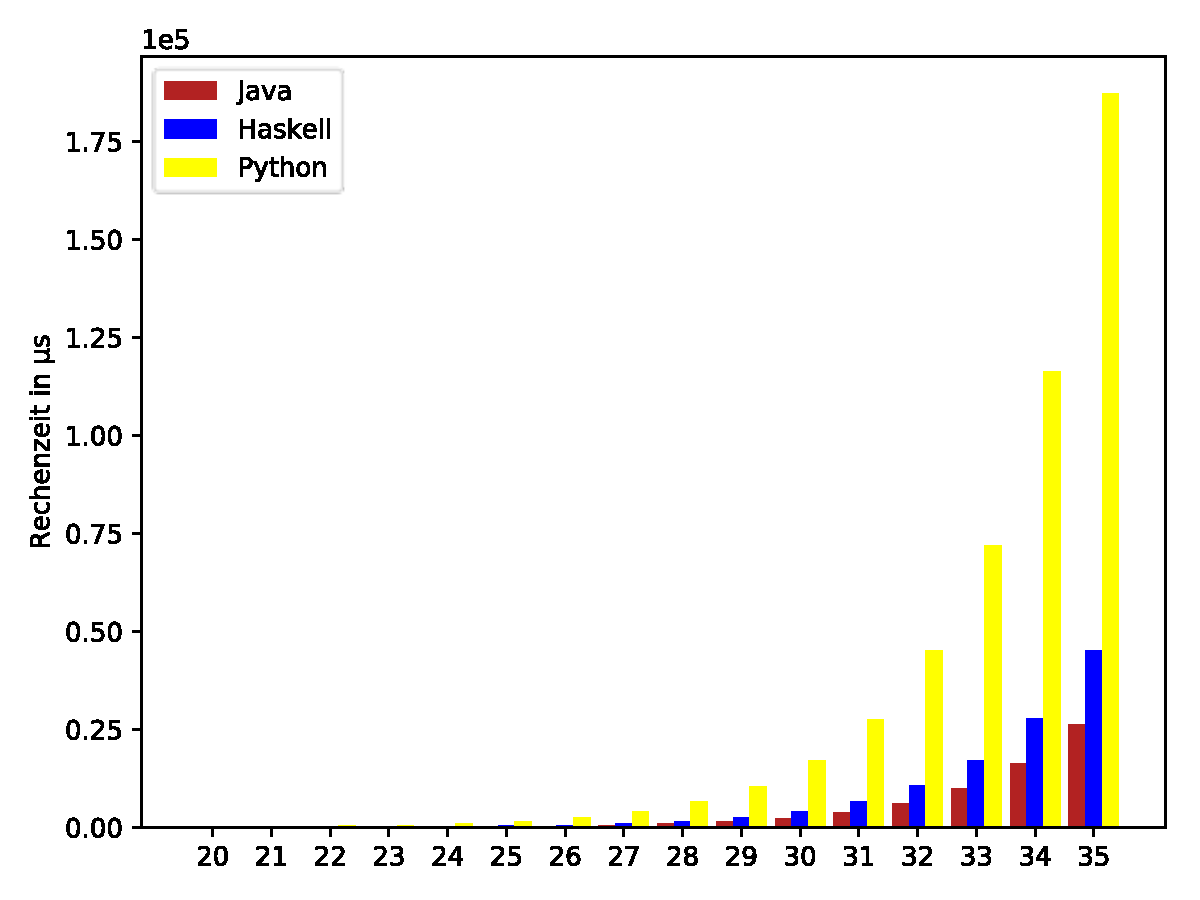
\includegraphics[width=\textwidth]{src/linear-microbench.pdf}
    \caption{Lineare Skala}
    \label{fig:micro-lin}
  \end{subfigure}%
  \begin{subfigure}{0.5\textwidth}
    \centering
    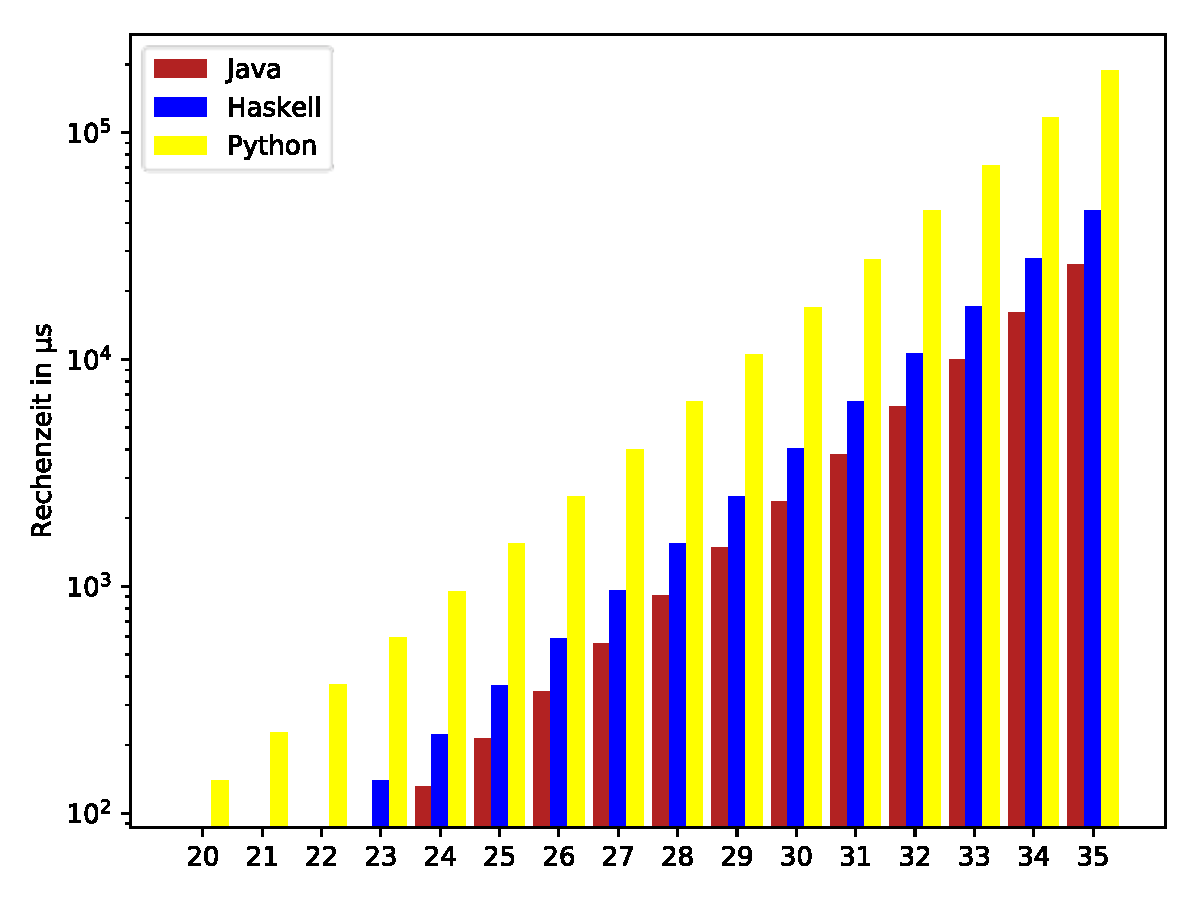
\includegraphics[width=\textwidth]{src/log-microbench.pdf}
    \caption{Logarithmische Skala}
    \label{fig:micro-log}
  \end{subfigure}
  \caption{Rechenzeiten von $fib(n)$ im Mikorbenchmark}
  \label{fig:micro}
\end{figure}

Wie in Abbildung~\ref{fig:micro-lin} zu sehen ist, benötigt der interpretierte Python-Code die meiste Rechenzeit.
Schneller ist der kompilierte Maschinencode von Haskell, welcher dennoch etwas langsamer ist als der Bytecode, der auf der JVM ausgeführt wird.
Zudem wird deutlich, dass die Rechenzeiten als Exponentialfunktion dargestellt werden können, was der theoretischen Laufzeitkomplexität des Algorithmus entspricht.

Auf einer logarithmischen Skala wird eine Exponentialfunktion der Form $f(x) = ae^{bx}$ auf eine lineare Funktion der Form $f'(x) = log(a) + bx * log(e)$ abgebildet.
Der Faktor $b$ kann vernachlässigt werden, da dieser die Anzahl der rekursiven Aufrufe bestimmt, welche bei jeder Implementierung identisch ist.
Die Basis $e$ ist in diesem Fall konstant und kann daher beim Vergleichen der Rechenzeiten vernachlässigt werden.
Also bleibt die Darstellung der Rechenzeiten in der Form $f'(x) = log(a) + x$.
Dadurch wird deutlich, dass die konstanten Abstände in Abbildung~\ref{fig:micro-log} zwischen den Rechenzeiten durch den X-Achsenabschnitt $log(a)$ - also den Faktor $a$ - verursacht werden.

In der Exponentialdarstellung ist der Faktor $a$ Teil der Basis, also ein konstanter Faktor, der bei jedem Funktionsaufruf auftritt.
Dies beweist, dass konstante Geschwindigkeitsunterschiede beim Ausführen der Rechenoperationen Ursache der unterschiedlichen Rechenzeiten sind.

\subsection{Ergebnisse des Benchmarks der eigenständigen Programme}

Die tatsächliche Laufzeit eines Programms hängt jedoch nicht alleine von der Zeit ab, die für das Ausführen der einzelnen Funktionen benötigt wird.
Weitere Faktoren, welche die Laufzeit bestimmen, sind das Laden des Programms, das Einrichten der Laufzeitumgebung und eventuelle Prüfungen sowie Optimierungen des ausgeführten Codes.

Um den Einfluss dieser anderen Faktoren zu bestimmen, werden die Funktionen aus den vorherigen Kapiteln in ein eigenständiges Programm verpackt, welches eine ganze Zahl als Programmparameter akzeptiert und diese als Argument für den Aufruf der Funktion $fib$ verwendet wird.
Zwar gibt es leichte Unterschiede in der Art, wie die gewählten Programmiersprachen, die Zeichenketten behandeln, über welche auf die Programmparameter zugegriffen werden kann, jedoch kann der Einfluss einer einzigen Umwandlung zu Programmstart angesichts der mehreren tausend Operationen während der Berechnung vernachlässigt werden.

Wird nun die Laufzeit für die Programme mit den selben Parametern des Mikrobenchmarks gemessen, entstehen die Messwerte aus Abbildung~\ref{fig:bench}.

\begin{figure}[h]
  \centering
  \begin{subfigure}{0.5\textwidth}
    \centering
    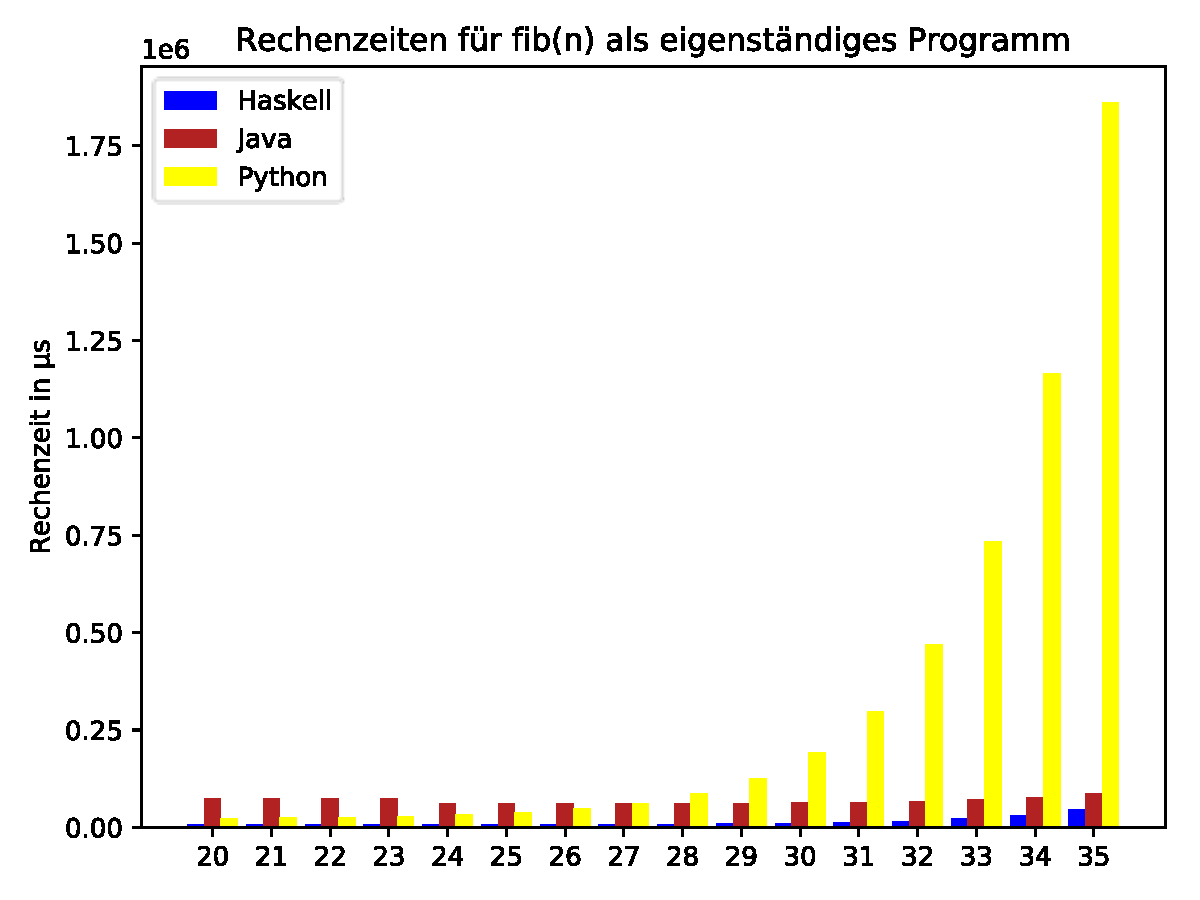
\includegraphics[width=\textwidth]{src/linear-standalone.pdf}
    \caption{Lineare Skala}
    \label{fig:bench-lin}
  \end{subfigure}%
  \begin{subfigure}{0.5\textwidth}
    \centering
    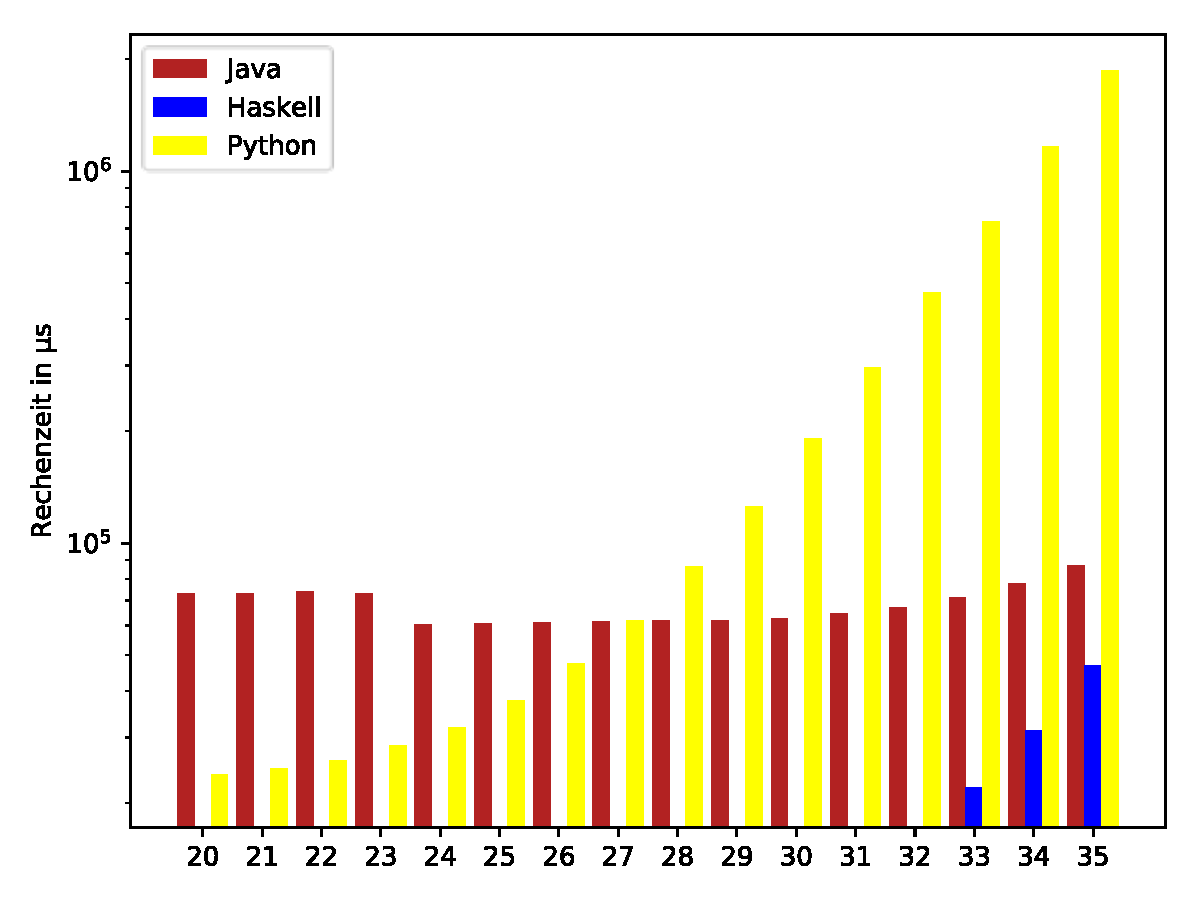
\includegraphics[width=\textwidth]{src/log-standalone.pdf}
    \caption{Logarithmische Skala}
    \label{fig:bench-log}
  \end{subfigure}
  \caption{Rechenzeiten von $fib(n)$ als eigenständiges Programm}
  \label{fig:bench}
\end{figure}


Sofort fallen in Abbildung~\ref{fig:bench-lin} Unterschiede zu den Rechenzeiten der einzelnen Funktionen aus Abbildung~\ref{fig:micro-lin} auf.
Haskell ist mit Abstand am schnellsten, wobei alle Fibonacci-Zahlen nahezu ohne Zeitaufwand berechnet werden.
In Abbildung~\ref{fig:bench-lin} zeigt die Rechenzeit des Java-Codes einen nahezu konstanten Verlauf auf.
Lediglich die Rechenzeit des interpretierten Python-Codes scheint erneut exponentiell zu verlaufen.

Auf der logarithmischen Skala in Abbildung~\ref{fig:bench-log} fällt auf, dass bei den Rechenzeiten des Python-Codes kein kontinuierlicher Anstieg der Rechenzeiten vorliegt.
Dies liegt an der konstanten Zeit, die durch das Laden des Programms und des Interpreters entsteht.
Da diese Zeit bei jeder Ausführung präsent ist, tritt für Berechnungen mit kleinen Eingabewerten der Aufwand für die tatsächliche Berechnung in den Hintergrund.
Dies bewirkt den zunächst flach ansteigenden Verlauf der Rechenzeiten.
Mit größer werdenden Eingabewerten überwiegt jedoch der Aufwand für die tatsächlichen Berechnungen, wodurch der typische exponentielle Verlauf entsteht.

Da beim Ausführen des kompilierten Haskell-Codes nahezu kein zusätzlicher Rechenaufwand entsteht, liegt weiterhin ein exponentieller Verlauf vor.
Die benötigte Rechenzeit wird dabei erst ab Eingabewerten von $n \ge 33$ so groß, dass sie der Zeit entspricht, die für das Laden des Python-Interpreters benötigt wird, wodurch die Rechenzeiten in Abbildung~\ref{fig:bench} kaum sichtbar erscheinen.

Auf einer exponentiellen Skala zeigt der Verlauf der von dem Java-Code benötigten Rechenzeiten
ein interessantes Verhalten.
Für Eingabewerte von $n = 20$ bis $n = 23$ ist ein leichter, kontinuierlicher Anstieg zu erkennen.
Ab $n = 24$ jedoch, ist die benötigte Rechenzeit wieder geringer und beginnt von dort an erneut zunehmend anzusteigen.
Grund für dieses Verhalten ist, dass statistische Optimierungen der JVM erst ab bestimmten Aufrufszahlen ausgeführt werden.
Wird eine Funktion sehr häufig aufgerufen, so kann der Just-in-time Mechanismus der JVM Aufrufe und deren Ergebnis zwischenspeichern.
Da $fib$ mit kleinzahligen Argumenten sehr häufig aufgerufen wird und die Funktion keine Seiteneffekte enthält, wird hier von der JVM das Ergebnis des Aufrufs zwischengespeichert, um eine erneute Berechnung zu vermeiden.
Durch diese Optimierung bleibt zwar die exponentielle Laufzeitkomplexität der Funktion erhalten, jedoch wird die Basis der Exponentialfunktion verringert, was dazu führt, dass die benötigte Zeit ebenso reduziert wird.

\section{Fazit}

Wie die Messergebnisse gezeigt haben, gibt es bei der Wahl eines Ausführungsmodells für die Implementierung einer Berechnung keine optimale Empfehlung.
Es jedoch ist erkennbar, dass mit zunehmendem Abstraktionsgrad die Rechengeschwindigkeit sinkt.
Deutlich wird dies am interpretierten Python-Code, bei dem durch den hohen Abstraktionsgrad einzelne Anweisungen nicht direkt in Maschinenanweisungen umgesetzt werden können.
Daher ist zu empfehlen, den Abstraktionsgrad nur so hoch zu wählen, wie es für die Implementierung nötig ist.
Weitere Abstraktionen führen nur zu Geschwindigkeitseinbußen bei der Ausführung.
Jedoch zeigen die Messergebnisse in dieser Arbeit, dass nicht etwa das maschinennahe Implementieren einer Berechnung den größten Einfluss auf die Rechenzeit hat, sondern die Optimierungen, die vor und während der Laufzeit angewandt werden können.
Dies wird bei der von Java benötigten Rechenzeit deutlich.
Die Laufzeitumgebung kann dort den ausgeführten Code während der Laufzeit optimieren, wodurch die benötigte Rechenzeit stark reduziert wird.
Durch diese Optimierungen wird sogar die Rechenzeit der kompilierten Maschineninstruktionen unterboten, welche herkömmlicherweise als schnellstes Ausführungsmodell gesehen werden.
Hierbei bewirkt der höhere Abstraktionsgrad von Java, dass es mehr Möglichkeiten zur Optimierung gibt.

Folglich bestimmt nicht die Wahl des Ausführungsmodells beim Implementieren einer Berechnung über die benötigte Rechenzeit.
Vielmehr sollte der Fokus darauf gelegt werden, dass die Quellsprache eine weite Reihe an Optimierungen unterstützt, welche die benötigte Rechenzeit verbessern.
Die positiven Auswirkungen von Optimierungen übersteigen dabei die kosten eines höheren Abstraktionsgrades.
Gerade wenn Berechnungen komplexer werden und über einen längeren Zeitraum laufen, kann die Zeit, die zum Initialisieren der Laufzeitumgebung benötigt wird, vernachlässigt werden.


\newpage

\bibliography{bib/bibtex}{}
\bibliographystyle{plain}

\end{document}



%%% Local Variables:
%%% mode: latex
%%% TeX-master: t
%%% End:
